% 默认页面大小 4:3
\documentclass[10pt]{ctexbeamer}
% 页面大小 16:10
% \documentclass[10pt, aspectratio=1610]{ctexbeamer}
% 页面大小 16:9
% \documentclass[10pt, aspectratio=169]{ctexbeamer}
% 页面大小 14:9
% \documentclass[10pt, aspectratio=149]{ctexbeamer}
% 页面大小 1.41:1
% \documentclass[10pt, aspectratio=141]{ctexbeamer}
% 页面大小 5:4
% \documentclass[10pt, aspectratio=54]{ctexbeamer}
% 页面大小 3:2
% \documentclass[10pt, aspectratio=32]{ctexbeamer}

\usetheme[logo=UCAS, sublogo=naoc]{ucas}
% logo 的选项: CAS, UCAS
% sublogo 的选项: AMSS, AMSS2018, UCAS

% 引入参考文献列表的 .bib 文件, 使用 GB/T 7714-2015 的文献著录规则.
\usepackage[backend=biber, style=gb7714-2015]{biblatex}
\addbibresource{ref.bib}

\title[UCAS Beamer (\LaTeX{})]{Transformer、时间序列模型以及论文精读}
% \subtitle[非官方]{非官方的模版}
\author[H. Zeng]{\href{mailto:haozeng1210@gmail.com}{曾滈}}
\institute[NAOC]{中国科学院国家天文台}
\date[\today]{\today, 北京怀柔}
\subject{展示主题}
\keywords{展示, 关键词}

\begin{document}

\begin{frame}[plain]
  \maketitle
\end{frame}

\begin{frame}[t]
  \frametitle{目录}
  \tableofcontents
\end{frame}

\section[transformer]{ 第1章 Transformer}\label{sec:1}
% \subsection[第 1 节缩写标题]{第 1 节标题}\label{subsec:1-1}


\begin{frame}[t]
  \frametitle{Transformer}
  从编码器解码器架构以及注意力机制到Transformer

  \begin{block}{编码器}
    编码器的任务是将输入向量$X$编码成中间语义表示$C$,通过非线性变换实现,即:
    \begin{equation}
      C = F(x_1, x_2, ..., x_n)
      \label{eq:编码器}
    \end{equation}
  \end{block}

  \begin{block}{解码器}
    解码器的职责在于根据中间语义表示$C$以及先前生成的历史信息$y_1, y_2, ..., y_{i-1}$,产生下一个词$y_i$,即:
    \begin{equation}
      y_i = G(y_1, y_2, ..., y_{i-1}, C)
      \label{eq:解码器}
    \end{equation}
  \end{block}
\end{frame}

\section[Time Series Models]{ 第2章 时间序列模型}\label{sec:2}



\begin{frame}[t]
  \frametitle{Time series}
  \begin{block}{时间序列模型}
    最近,预训练模型,特别是基于Transformer的预训练模型在计算机视觉和自然语言处理等领域取得了卓越的性能。受此启发,近来的研究开始考虑时间序列的预训练模型的设计。\\

    首先,通过有监督、无监督和自监督学习对模型进行训练来获取恰当的表示,然后模型在目标领域进行微调以求在下游的时间序列任务(例如时间序列分类以及异常检测)中获得性能提升。
  \end{block}
\end{frame}


\begin{frame}[t]
  \frametitle{模型分类}
  \begin{figure}
    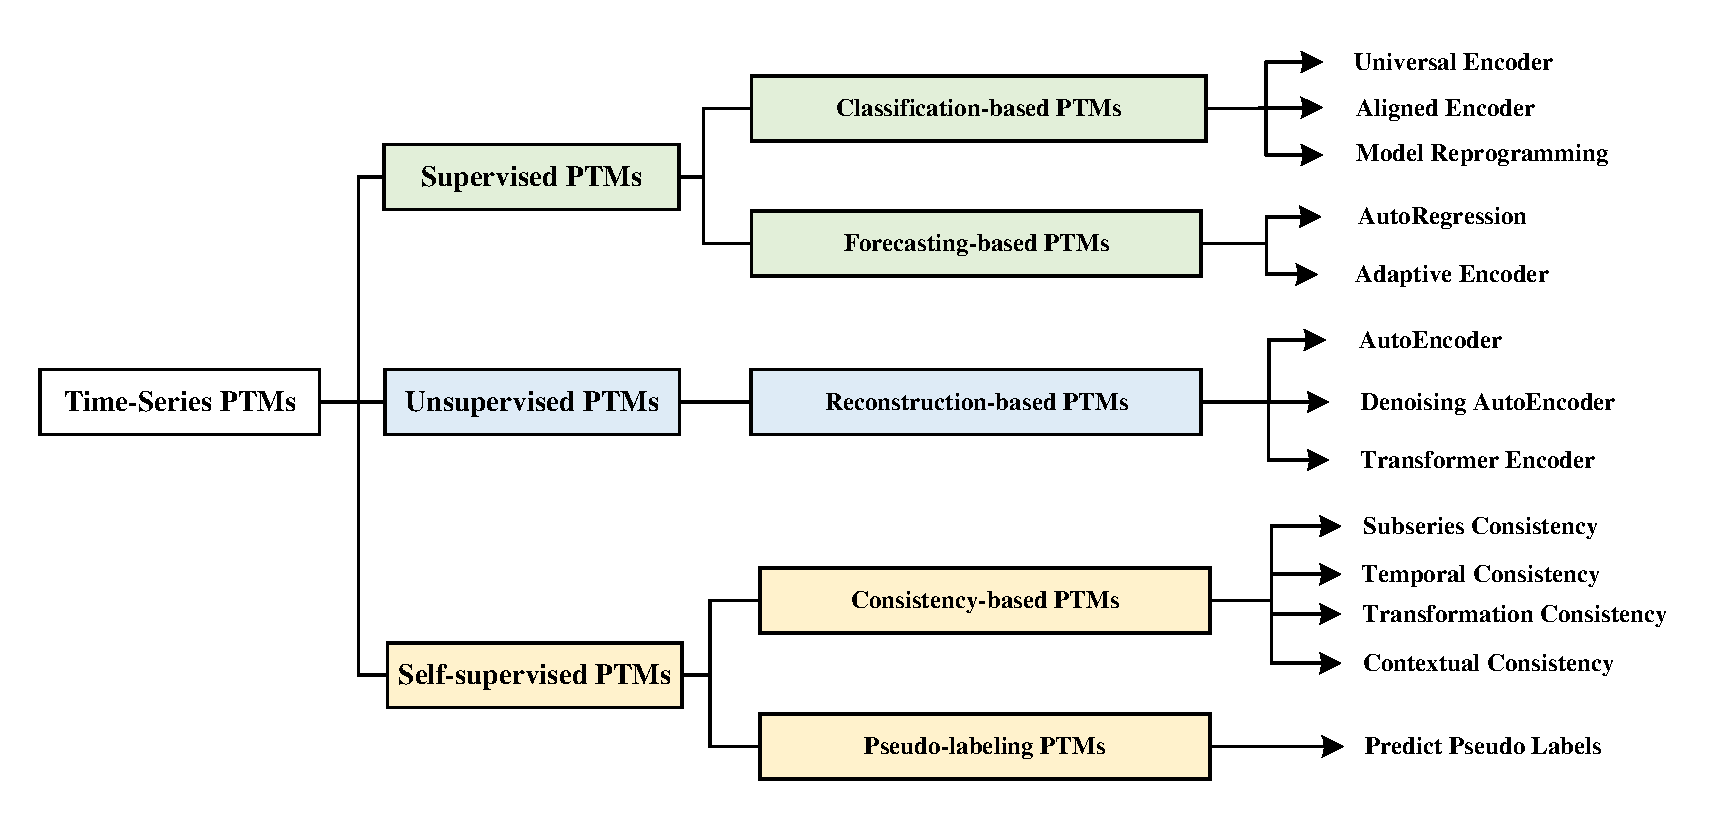
\includegraphics[width=.8\textwidth, height=.8\textheight, keepaspectratio]{taxonomy.pdf}
    \caption{基于训练技巧和任务对模型分类}
  \end{figure}
\end{frame}

\section[AstroLLaMA]{ 第3章 AstroLLaMA}\label{sec:3}



\begin{frame}[t]
  \frametitle{研究背景和动机}
  \begin{itemize}
    \item 预训练语言模型(LLM)在通用任务上表现出色,但在天文学等专业领域上效果不佳。
    \item 天文领域数据相对较少,导致LLM在此领域知识建模效果不佳,存在hallucination等问题。
    \item 天文领域专用LLM较少,如astroBERT,但参数较少。
  \end{itemize}
\end{frame}

\begin{frame}[t]
  \frametitle{模型构建}
  \begin{itemize}
    \item 基于LLaMA-2模型,使用300,000+篇arXiv论文摘要进行微调。
    \item 数据集处理和模型参数设定。
    \item 微调后的模型在天文领域的适应性得到了验证,perplexity指标降低了32.5%。
  \end{itemize}
\end{frame}

\begin{frame}[t]
  \frametitle{模型评估}
  \begin{itemize}
    \item 模型在文本生成和embedding空间质量上进行评估。
    \item 与LLaMA-2/GPT-4对比,AstroLLaMA能生成更加专业和准确的文本。
    \item embedding空间显示了更强的语义建模能力。
  \end{itemize}
\end{frame}

\begin{frame}[t]
  \frametitle{创新点和意义}
  \begin{itemize}
    \item 提出了首个大规模的天文LLM。
    \item 验证了专用微调的有效性。
    \item 开放了模型权重,为天文AI研究开启了新的可能性。
  \end{itemize}
\end{frame}

\begin{frame}[t]
  \frametitle{当前局限和未来工作}
  \begin{itemize}
    \item 模型在某些领域知识上仍有缺陷。
    \item 模型在生成数据时可能会产生不准确的数值。
    \item 公开模型的目的是鼓励社区的参与,提高模型的准确性和创造性。
  \end{itemize}
\end{frame}



\begin{frame}[noframenumbering, allowframebreaks, t]
  \frametitle{参考文献}
  \nocite{*}% 打印未引用,但已列入 .bib 文件内的文献
  \printbibliography%
\end{frame}

\begin{frame}[plain]
  \vfill
  \centerline{\Huge 谢谢}
  \vfill
\end{frame}

\end{document}
